\documentclass{scrartcl}
\usepackage[margin=3cm]{geometry}
\usepackage{amsmath}
\usepackage{amssymb}
\usepackage{amsthm}
\usepackage{blindtext}
\usepackage{datetime}
\usepackage{fontspec}
\usepackage{float}
\usepackage{graphicx}
\usepackage{kotex}
\usepackage[lighttt]{lmodern}
\usepackage{listings}
\usepackage{mathrsfs}
\usepackage{mathtools}
\usepackage{pgf,tikz,pgfplots}

\pgfplotsset{compat=1.15}
\usetikzlibrary{arrows}
\newtheorem{theorem}{Theorem}

\lstset{
  numbers=none, frame=single, showspaces=false,
  showstringspaces=false, showtabs=false, breaklines=true, showlines=true,
  breakatwhitespace=true, basicstyle=\ttfamily, keywordstyle=\bfseries, basewidth=0.5em
}

\setmainhangulfont{Noto Serif CJK KR}[
  UprightFont=* Light, BoldFont=* Bold,
  Script=Hangul, Language=Korean, AutoFakeSlant,
]
\setsanshangulfont{Noto Sans CJK KR}[
  UprightFont=* DemiLight, BoldFont=* Medium,
  Script=Hangul, Language=Korean
]
\setmathhangulfont{Noto Sans CJK KR}[
  SizeFeatures={
    {Size=-6,  Font=* Medium},
    {Size=6-9, Font=*},
    {Size=9-,  Font=* DemiLight},
  },
  Script=Hangul, Language=Korean
]
\title{디지털시스템설계 Lab 6}
\author{손량(20220323)}
\date{Last compiled on: \today, \currenttime}

\newcommand{\un}[1]{\ensuremath{\ \mathrm{#1}}}

\begin{document}
\maketitle

\section{개요}
수업 시간에 배운 counter를 베릴로그 코드로 구현하고 시뮬레이션을 수행해 본다.

\section{이론적 배경}
\subsection{D Flip-Flop}
D flip-flop은 클럭 신호에 따라 \(D\) 입력에 맞추어 \(Q\)가 반영되는 회로이다.
Excitation table은 다음과 같이 그릴 수 있다.
\begin{table}[H]
  \centering
  \begin{tabular}{ll|l}
    \hline
    \(D\) & \(Q\) & \(Q^+\) \\
    \hline
    0 & 0 & 0 \\
    0 & 1 & 0 \\
    1 & 0 & 1 \\
    1 & 1 & 1 \\
    \hline
  \end{tabular}
\end{table}

\subsection{Counter}
Counter는 clock 신호에 맞춰 미리 정의된 규칙에 따라 데이터를 저장하고 출력한다.

\subsubsection{Synchronous Counter}
모든 flip-flop에 클럭 신호가 동시에 입력되는 회로를 synchronous counter라고 부른다.
Flip-flop에 의한 clock delay가 없기 때문에 속도가 빠르지만, 회로가 더 복잡하다는 단점이 존재한다.

\subsubsection{Decade Counter}
Decade counter는 10진수의 숫자 0, 1, 2, 3, 4, 5, 6, 7, 8, 9를 순차적으로 세는 회로이다.

\section{실험 준비}
\subsection{Synchronous Decade BCD Counter}
\subsubsection{State Diagram}
State diagram은 다음과 같이 그릴 수 있다.
\begin{figure}[H]
  \centering
  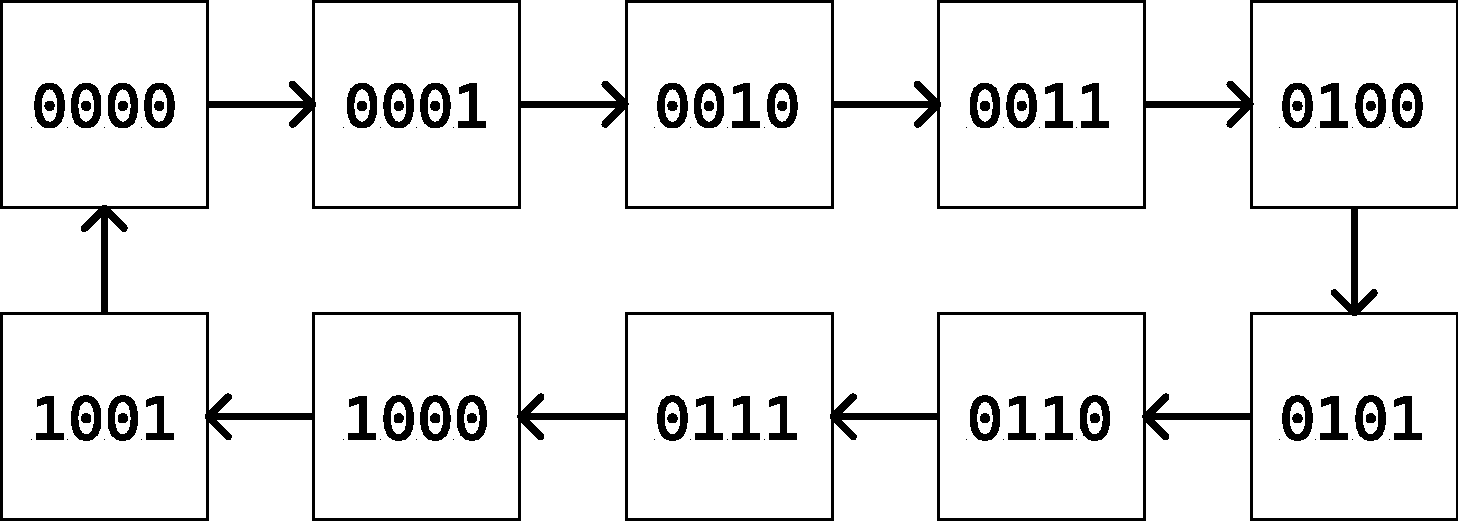
\includegraphics[width=0.7\linewidth]{lab6_1_states.pdf}
\end{figure}

\subsubsection{State Transition Table}
State transition diagram과 JK flip-flop의 입력은 다음과 같다.
\begin{table}[H]
  \centering
  \begin{tabular}{cccc|cccc|cc|cc|cc|cc}
    \hline
    \(Q_3\) & \(Q_2\) & \(Q_1\) & \(Q_0\) & \(Q^+_3\) & \(Q^+_2\) & \(Q^+_1\) & \(Q^+_0\) & \(J_3\) & \(K_3\) & \(J_2\) & \(K_2\) & \(J_1\) & \(K_1\) & \(J_0\) & \(K_0\) \\
    \hline
    0 & 0 & 0 & 0 & 0 & 0 & 0 & 1 & 0 & X & 0 & X & 0 & X & 1 & X \\
    0 & 0 & 0 & 1 & 0 & 0 & 1 & 0 & 0 & X & 0 & X & 1 & X & X & 1 \\
    0 & 0 & 1 & 0 & 0 & 0 & 1 & 1 & 0 & X & 0 & X & X & 0 & 1 & X \\
    0 & 0 & 1 & 1 & 0 & 1 & 0 & 0 & 0 & X & 1 & X & X & 1 & X & 1 \\
    0 & 1 & 0 & 0 & 0 & 1 & 0 & 1 & 0 & X & X & 0 & 0 & X & 1 & X \\
    0 & 1 & 0 & 1 & 0 & 1 & 1 & 0 & 0 & X & X & 0 & 1 & X & X & 1 \\
    0 & 1 & 1 & 0 & 0 & 1 & 1 & 1 & 0 & X & X & 0 & X & 0 & 1 & X \\
    0 & 1 & 1 & 1 & 1 & 0 & 0 & 0 & 1 & X & X & 1 & X & 1 & X & 1 \\
    1 & 0 & 0 & 0 & 1 & 0 & 0 & 1 & X & 0 & 0 & X & 0 & X & 1 & X \\
    1 & 0 & 0 & 1 & 0 & 0 & 0 & 0 & X & 1 & 0 & X & 0 & X & X & 1 \\
    1 & 0 & 1 & 0 & - & - & - & - & X & X & X & X & X & X & X & X \\
    1 & 0 & 1 & 1 & - & - & - & - & X & X & X & X & X & X & X & X \\
    1 & 1 & 0 & 0 & - & - & - & - & X & X & X & X & X & X & X & X \\
    1 & 1 & 0 & 1 & - & - & - & - & X & X & X & X & X & X & X & X \\
    1 & 1 & 1 & 0 & - & - & - & - & X & X & X & X & X & X & X & X \\
    1 & 1 & 1 & 1 & - & - & - & - & X & X & X & X & X & X & X & X \\
    \hline
  \end{tabular}
\end{table}

\(J,\, K\) 입력의 K-map을 그리면
\begin{figure}[H]
  \centering
  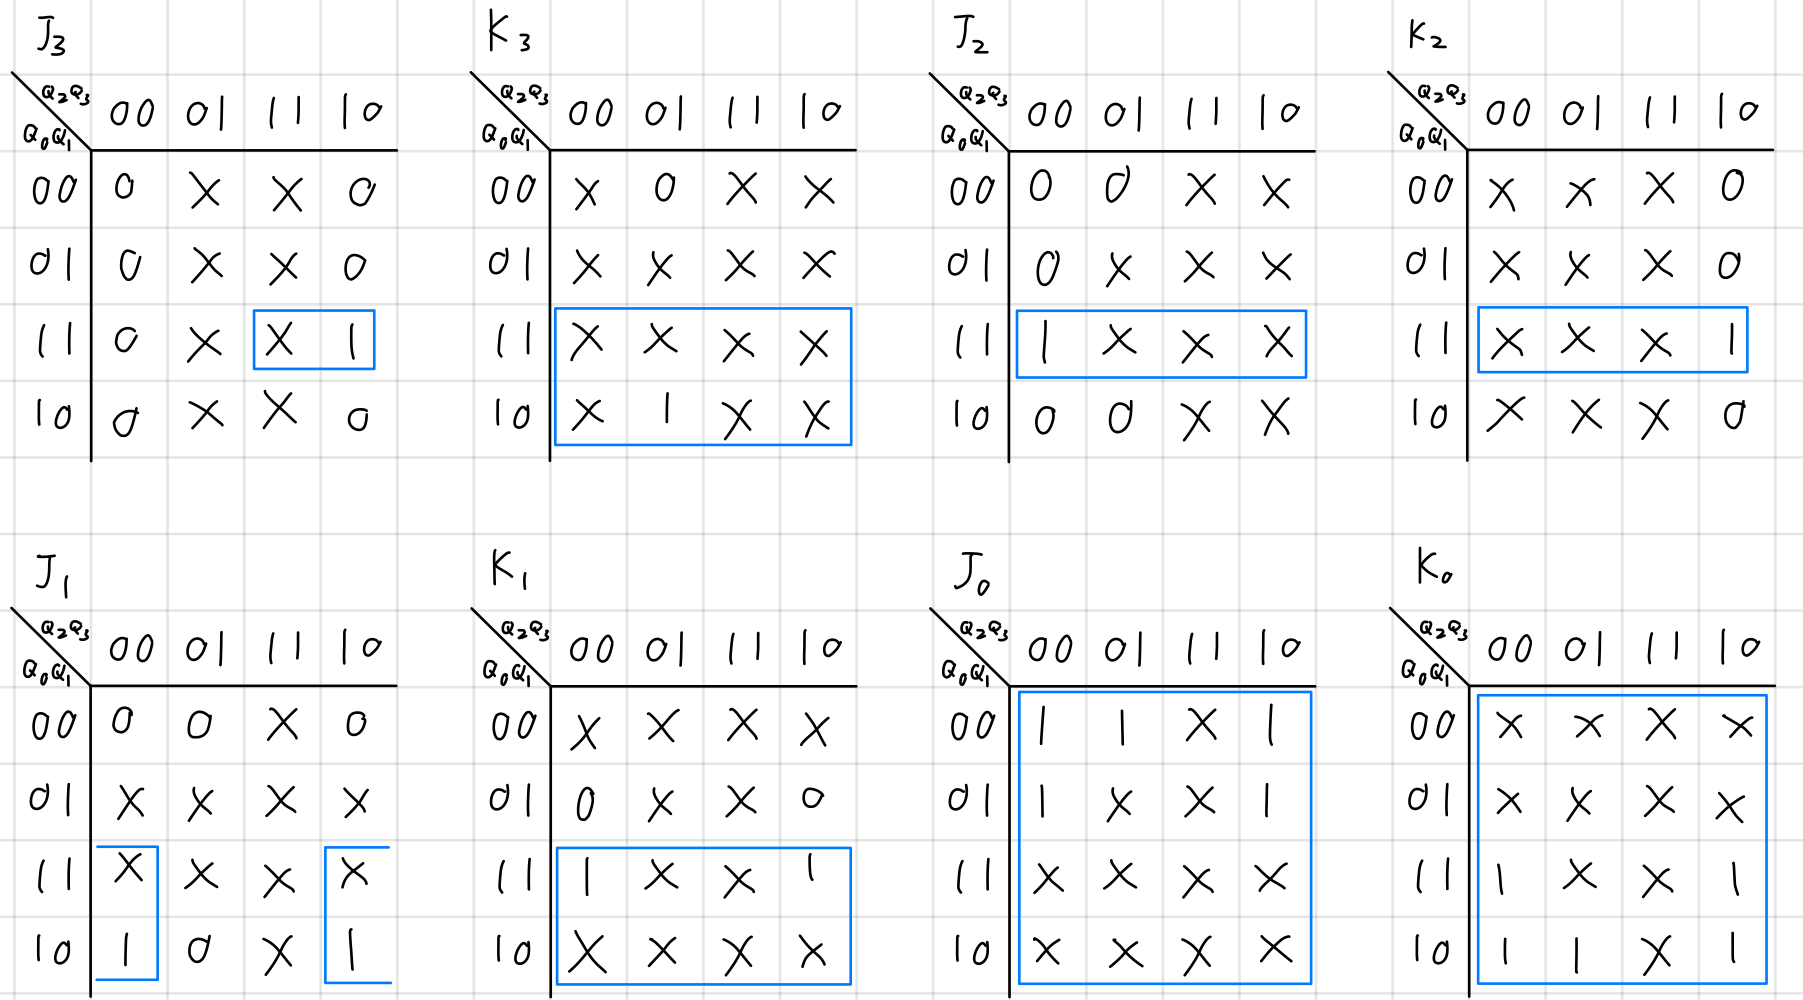
\includegraphics[width=0.9\linewidth]{lab6_1_kmap.jpeg}
\end{figure}
단순화하면
\begin{align*}
  J_0 &= 1 \quad K_0 = 1 \\
  J_1 &= Q_0 Q_3' \quad K_1 = Q_0 \\
  J_2 &= Q_0 Q_1 \quad K_2 = Q_0 Q_1 \\
  J_3 &= Q_0 Q_1 Q_2 \quad K_3 = Q_0
\end{align*}

\subsubsection{Circuit Diagram}
회로도는 다음과 같다.
\begin{figure}[H]
  \centering
  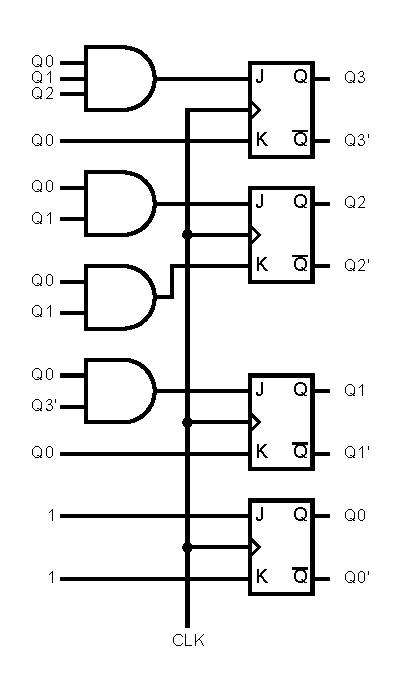
\includegraphics[width=0.5\linewidth]{lab6_1_circuit.pdf}
\end{figure}

\subsection{Synchronous Decade BCD Counter (두 자릿수)}
\subsubsection{State Diagram}
State transition diagram은 다음과 같다.
\begin{table}[H]
  \centering
  \begin{tabular}{cccccccc|cccccccc}
    \hline
    \(Q_7\) & \(Q_6\) & \(Q_5\) & \(Q_4\) & \(Q_3\) & \(Q_2\) & \(Q_1\) & \(Q_0\) & \(Q^+_7\) & \(Q^+_6\) & \(Q^+_5\) & \(Q^+_4\) & \(Q^+_3\) & \(Q^+_2\) & \(Q^+_1\) & \(Q^+_0\) \\
    \hline
    0 & 0 & 0 & 0 & 0 & 0 & 0 & 0 & 0 & 0 & 0 & 0 & 0 & 0 & 0 & 1 \\
    0 & 0 & 0 & 0 & 0 & 0 & 0 & 1 & 0 & 0 & 0 & 0 & 0 & 0 & 1 & 0 \\
    0 & 0 & 0 & 0 & 0 & 0 & 1 & 0 & 0 & 0 & 0 & 0 & 0 & 0 & 1 & 1 \\
    0 & 0 & 0 & 0 & 0 & 0 & 1 & 1 & 0 & 0 & 0 & 0 & 0 & 1 & 0 & 0 \\
    0 & 0 & 0 & 0 & 0 & 1 & 0 & 0 & 0 & 0 & 0 & 0 & 0 & 1 & 0 & 1 \\
    0 & 0 & 0 & 0 & 0 & 1 & 0 & 1 & 0 & 0 & 0 & 0 & 0 & 1 & 1 & 0 \\
    0 & 0 & 0 & 0 & 0 & 1 & 1 & 0 & 0 & 0 & 0 & 0 & 0 & 1 & 1 & 1 \\
    0 & 0 & 0 & 0 & 0 & 1 & 1 & 1 & 0 & 0 & 0 & 0 & 1 & 0 & 0 & 0 \\
    0 & 0 & 0 & 0 & 1 & 0 & 0 & 0 & 0 & 0 & 0 & 0 & 1 & 0 & 0 & 1 \\
    0 & 0 & 0 & 0 & 1 & 0 & 0 & 1 & 0 & 0 & 0 & 1 & 0 & 0 & 0 & 0 \\
    0 & 0 & 0 & 0 & 1 & 0 & 1 & 0 & - & - & - & - & - & - & - & - \\
    0 & 0 & 0 & 0 & 1 & 0 & 1 & 1 & - & - & - & - & - & - & - & - \\
    0 & 0 & 0 & 0 & 1 & 1 & 0 & 0 & - & - & - & - & - & - & - & - \\
    0 & 0 & 0 & 0 & 1 & 1 & 0 & 1 & - & - & - & - & - & - & - & - \\
    0 & 0 & 0 & 0 & 1 & 1 & 1 & 0 & - & - & - & - & - & - & - & - \\
    0 & 0 & 0 & 0 & 1 & 1 & 1 & 1 & - & - & - & - & - & - & - & - \\
    0 & 0 & 0 & 1 & 0 & 0 & 0 & 0 & 0 & 0 & 0 & 1 & 0 & 0 & 0 & 1 \\
    \vdots & \vdots & \vdots & \vdots & \vdots & \vdots & \vdots & \vdots & \vdots & \vdots & \vdots & \vdots & \vdots & \vdots & \vdots & \vdots \\
    0 & 0 & 0 & 1 & 1 & 0 & 0 & 0 & 0 & 0 & 0 & 1 & 1 & 0 & 0 & 1 \\
    0 & 0 & 0 & 1 & 1 & 0 & 0 & 1 & 0 & 0 & 1 & 0 & 0 & 0 & 0 & 0 \\
    0 & 0 & 0 & 1 & 1 & 0 & 1 & 0 & - & - & - & - & - & - & - & - \\
    0 & 0 & 0 & 1 & 1 & 0 & 1 & 1 & - & - & - & - & - & - & - & - \\
    0 & 0 & 0 & 1 & 1 & 1 & 0 & 0 & - & - & - & - & - & - & - & - \\
    0 & 0 & 0 & 1 & 1 & 1 & 0 & 1 & - & - & - & - & - & - & - & - \\
    0 & 0 & 0 & 1 & 1 & 1 & 1 & 0 & - & - & - & - & - & - & - & - \\
    0 & 0 & 0 & 1 & 1 & 1 & 1 & 1 & - & - & - & - & - & - & - & - \\
    \vdots & \vdots & \vdots & \vdots & \vdots & \vdots & \vdots & \vdots & \vdots & \vdots & \vdots & \vdots & \vdots & \vdots & \vdots & \vdots \\
    1 & 0 & 0 & 1 & 0 & 0 & 0 & 0 & 1 & 0 & 0 & 1 & 0 & 0 & 0 & 1 \\
    \vdots & \vdots & \vdots & \vdots & \vdots & \vdots & \vdots & \vdots & \vdots & \vdots & \vdots & \vdots & \vdots & \vdots & \vdots & \vdots \\
    1 & 0 & 0 & 1 & 1 & 0 & 0 & 0 & 1 & 0 & 0 & 1 & 1 & 0 & 0 & 1 \\
    1 & 0 & 0 & 1 & 1 & 0 & 0 & 1 & 0 & 0 & 0 & 0 & 0 & 0 & 0 & 0 \\
    1 & 0 & 0 & 1 & 1 & 0 & 1 & 0 & - & - & - & - & - & - & - & - \\
    1 & 0 & 0 & 1 & 1 & 0 & 1 & 1 & - & - & - & - & - & - & - & - \\
    1 & 0 & 0 & 1 & 1 & 1 & 0 & 0 & - & - & - & - & - & - & - & - \\
    1 & 0 & 0 & 1 & 1 & 1 & 0 & 1 & - & - & - & - & - & - & - & - \\
    1 & 0 & 0 & 1 & 1 & 1 & 1 & 0 & - & - & - & - & - & - & - & - \\
    1 & 0 & 0 & 1 & 1 & 1 & 1 & 1 & - & - & - & - & - & - & - & - \\
    \hline
  \end{tabular}
\end{table}

\subsubsection{Circuit Diagram}
회로도는 다음과 같다.
\begin{figure}[H]
  \centering
  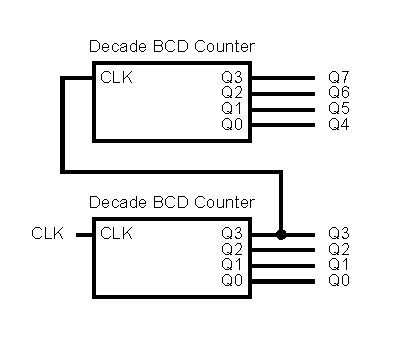
\includegraphics[width=0.4\linewidth]{lab6_2_circuit.pdf}
\end{figure}

\subsection{369 계수기}
\subsubsection{State Diagram}
State diagram은 다음과 같이 그릴 수 있다.
\begin{figure}[H]
  \centering
  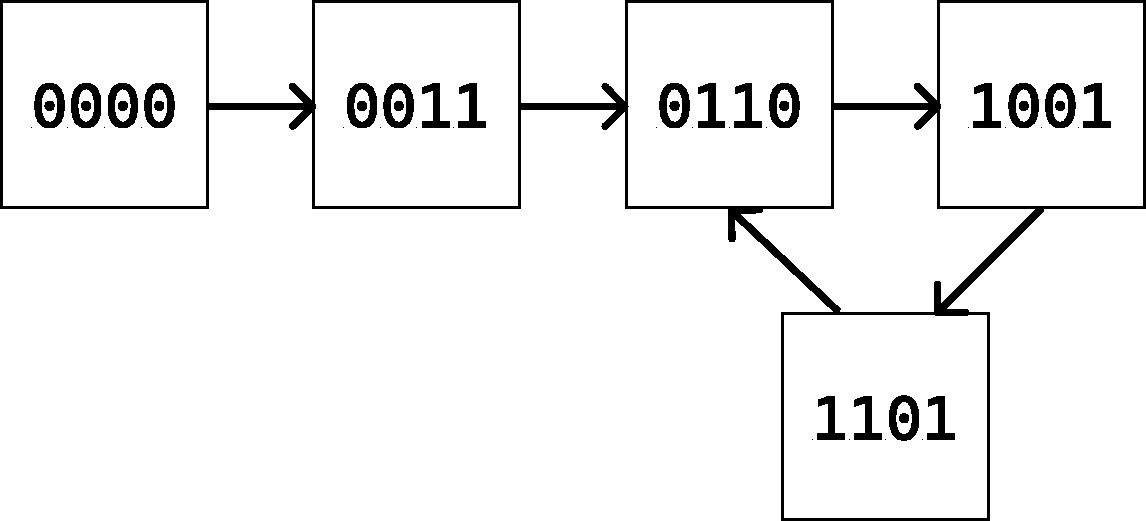
\includegraphics[width=0.5\linewidth]{lab6_3_states.pdf}
\end{figure}

\subsubsection{State Transition Table}
State transition diagram은 다음과 같다.
\begin{table}[H]
  \centering
  \begin{tabular}{cccc|cccc|cccc}
    \hline
    \(Q_3\) & \(Q_2\) & \(Q_1\) & \(Q_0\) & \(Q^+_3\) & \(Q^+_2\) & \(Q^+_1\) & \(Q^+_0\) & \(D_3\) & \(D_2\) & \(D_1\) & \(D_0\) \\
    \hline
    0 & 0 & 0 & 0 & 0 & 0 & 1 & 1 & 0 & 0 & 1 & 1 \\
    0 & 0 & 0 & 1 & - & - & - & - & X & X & X & X \\
    0 & 0 & 1 & 0 & - & - & - & - & X & X & X & X \\
    0 & 0 & 1 & 1 & 0 & 1 & 1 & 0 & 0 & 1 & 1 & 0 \\
    0 & 1 & 0 & 0 & - & - & - & - & X & X & X & X \\
    0 & 1 & 0 & 1 & - & - & - & - & X & X & X & X \\
    0 & 1 & 1 & 0 & 1 & 0 & 0 & 1 & 1 & 0 & 0 & 1 \\
    0 & 1 & 1 & 1 & - & - & - & - & X & X & X & X \\
    1 & 0 & 0 & 0 & - & - & - & - & X & X & X & X \\
    1 & 0 & 0 & 1 & 1 & 1 & 0 & 1 & 1 & 1 & 0 & 1 \\
    1 & 0 & 1 & 0 & - & - & - & - & X & X & X & X \\
    1 & 0 & 1 & 1 & - & - & - & - & X & X & X & X \\
    1 & 1 & 0 & 0 & - & - & - & - & X & X & X & X \\
    1 & 1 & 0 & 1 & 0 & 1 & 1 & 0 & 0 & 1 & 1 & 0 \\
    1 & 1 & 1 & 0 & - & - & - & - & X & X & X & X \\
    1 & 1 & 1 & 1 & - & - & - & - & X & X & X & X \\
    \hline
  \end{tabular}
\end{table}
\(D\) 입력의 K-map을 그리면
\begin{figure}[H]
  \centering
  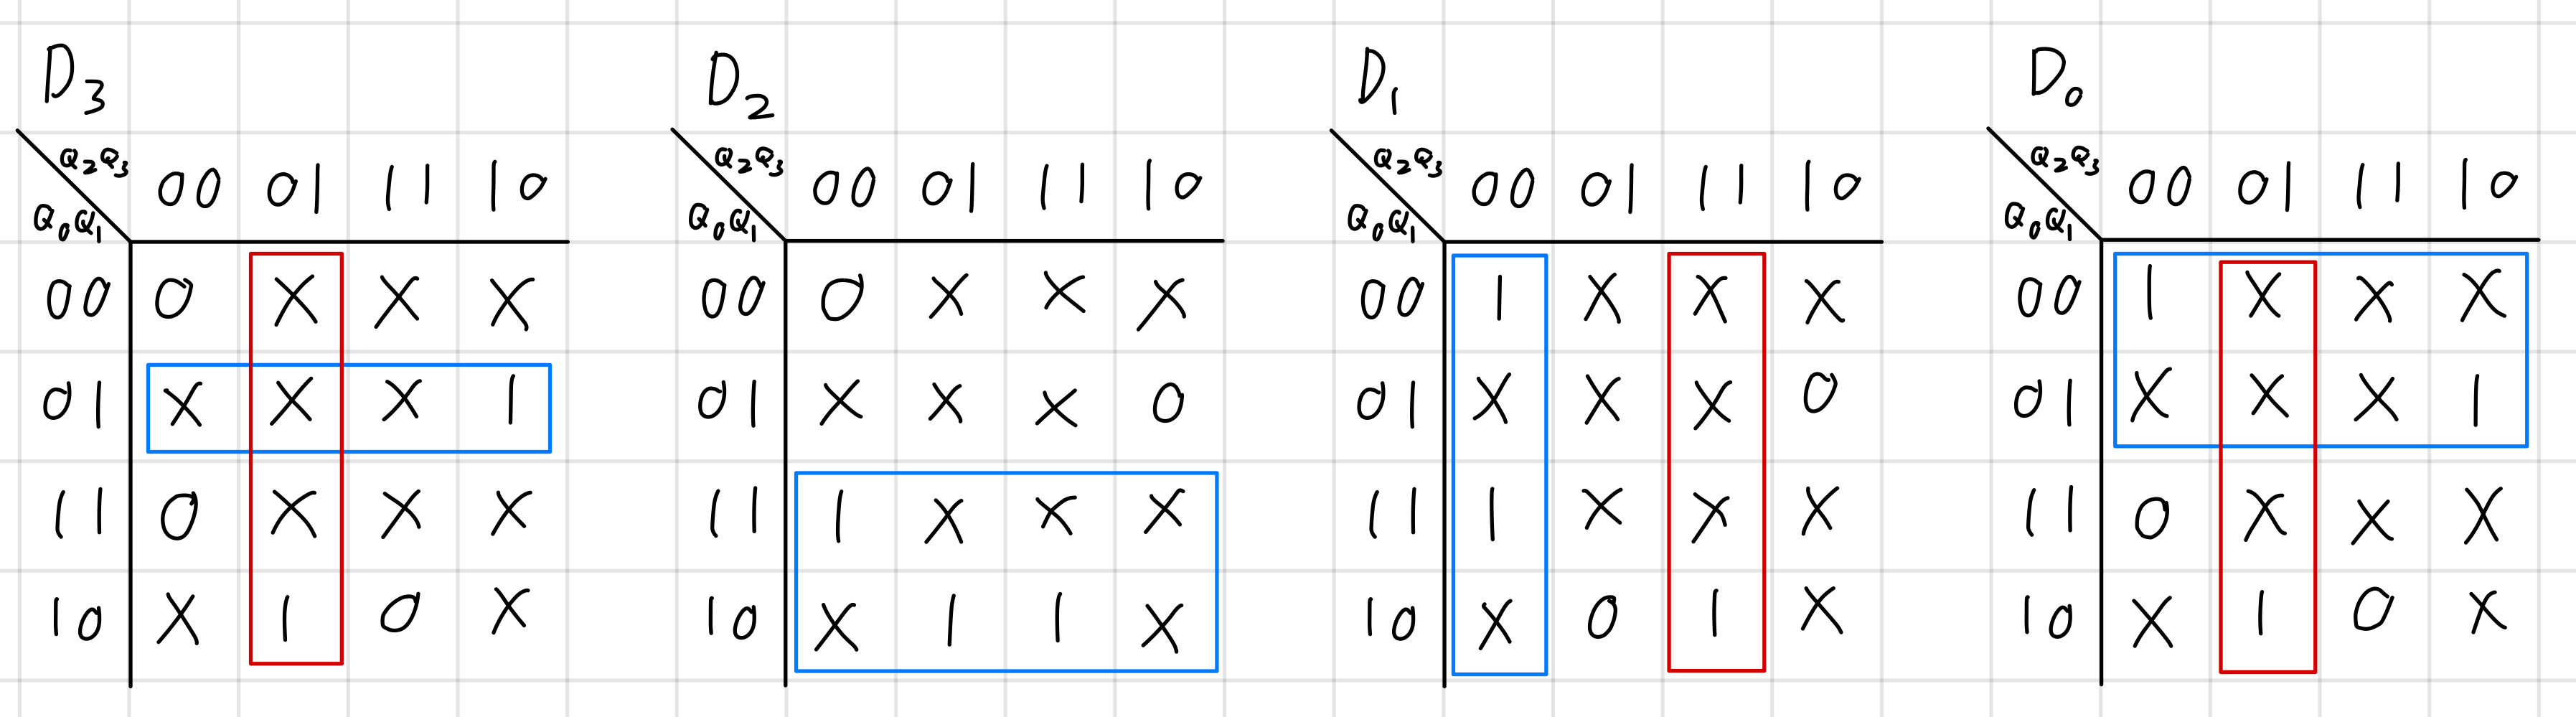
\includegraphics[width=0.9\linewidth]{lab6_3_kmap.jpeg}
\end{figure}
단순화하면
\begin{align*}
  D_0 &= Q_0' + Q_2' Q_3 \\
  D_1 &= Q_2' Q_3' + Q_2 Q_3 \\
  D_2 &= Q_0 \\
  D_3 &= Q_0' Q_1 + Q_2' Q_3
\end{align*}

\subsubsection{Circuit Diagram}
회로도는 다음과 같다.
\begin{figure}[H]
  \centering
  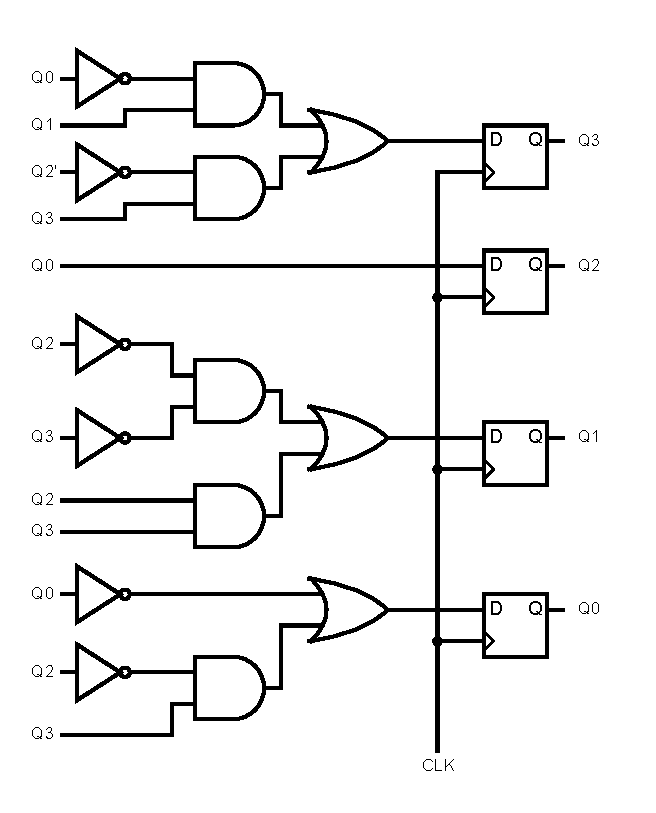
\includegraphics[width=0.6\linewidth]{lab6_3_circuit.pdf}
\end{figure}

\section{실험 결과}
우선 \texttt{lab6\_tb.v}에서 생성된 전체 파형은 다음과 같다.
\begin{figure}[H]
  \centering
  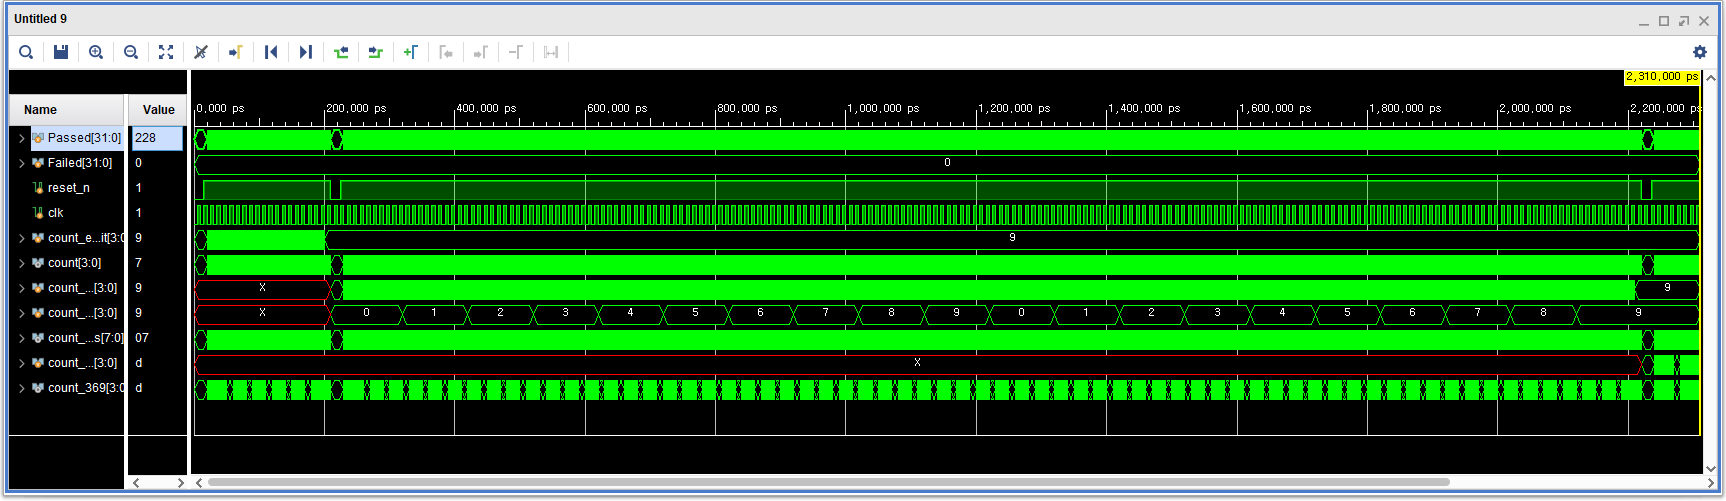
\includegraphics[width=0.9\linewidth]{lab6_waveform.png}
\end{figure}

\subsection{\texttt{lab6\_1.v} -- Synchronous Decade BCD Counter}
Vivado에서 생성된 회로는 다음과 같다.
\begin{figure}[H]
  \centering
  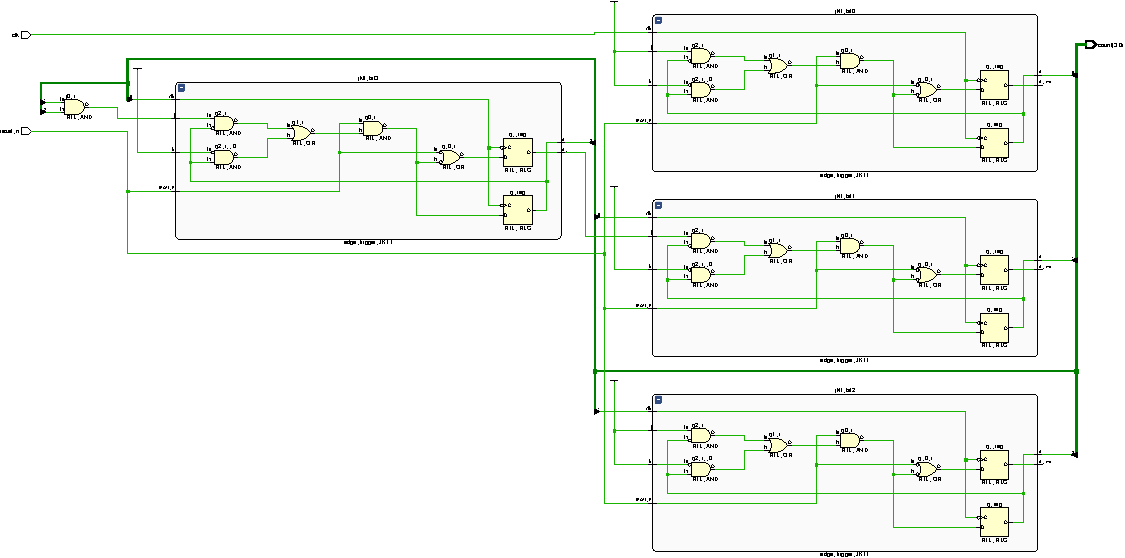
\includegraphics[width=0.9\linewidth]{lab6_1_schematic-crop.pdf}
\end{figure}

테스트벤치 실행 결과 중 \texttt{lab6\_1.v}와 관계있는 부분은 다음과 같다.
\begin{figure}[H]
  \centering
  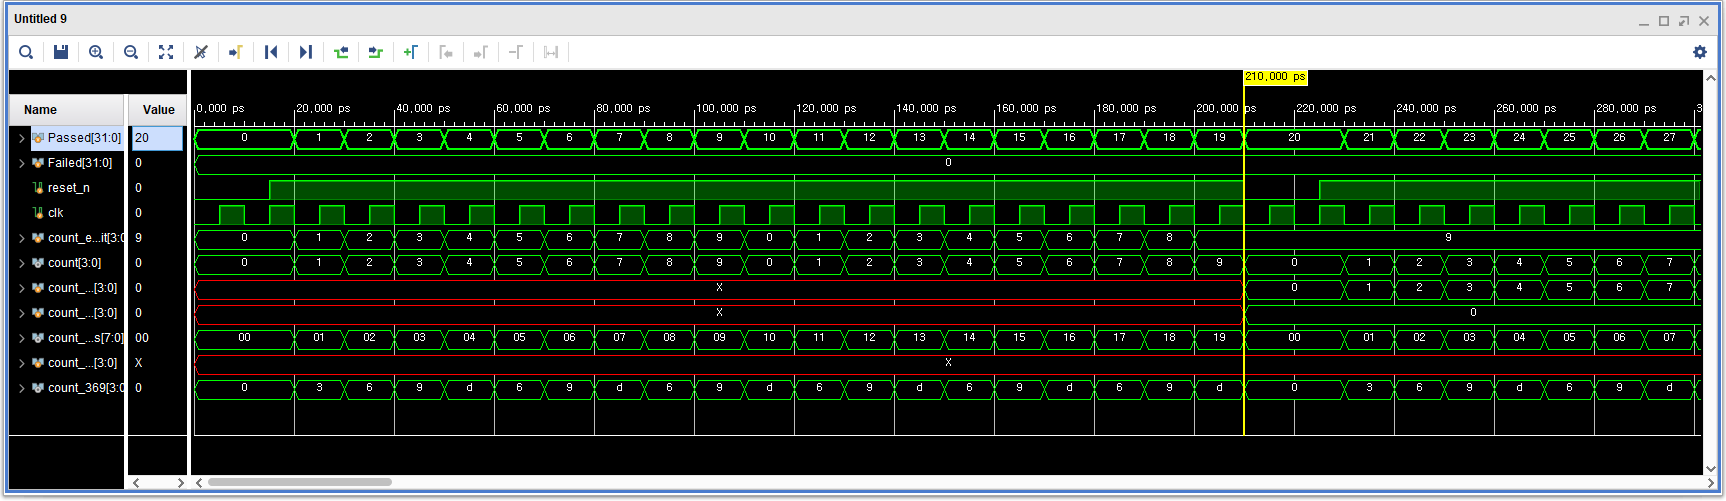
\includegraphics[width=0.9\linewidth]{lab6_1_waveform.png}
\end{figure}
0부터 시작해서 9에 도달한 다음 다시 0으로 돌아가는 정상 작동을 함을 알 수 있다.

\subsection{\texttt{lab6\_2.v} -- Synchronous Decade BCD Counter (두 자릿수)}
Vivado에서 생성된 회로는 다음과 같다.
\begin{figure}[H]
  \centering
  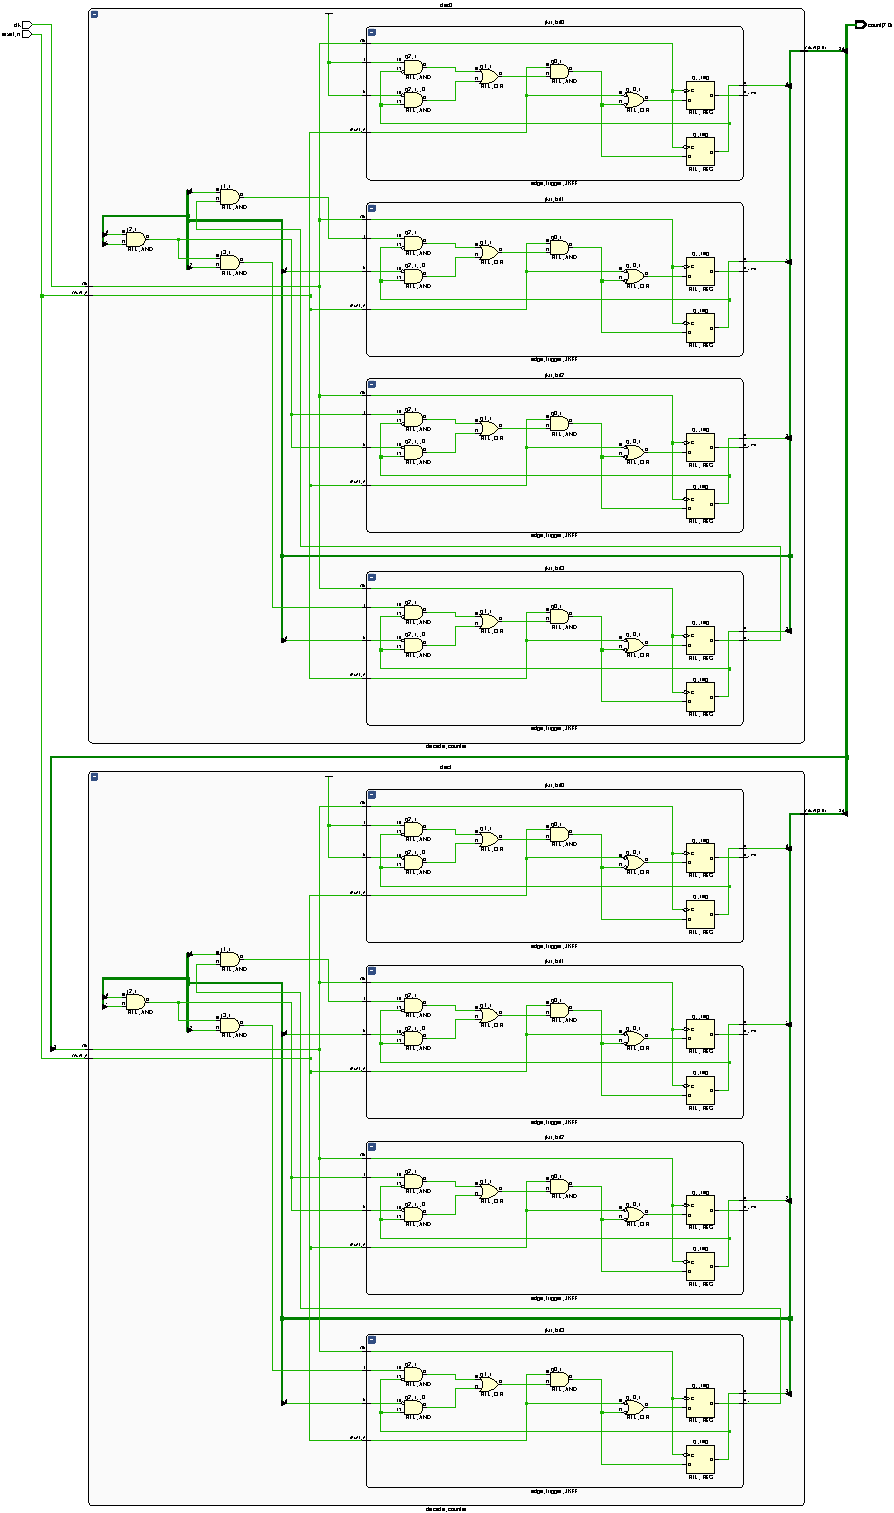
\includegraphics[width=0.9\linewidth]{lab6_2_schematic-crop.pdf}
\end{figure}

테스트벤치 실행 결과 중 \texttt{lab6\_2.v}와 관계있는 부분은 다음과 같다.
\begin{figure}[H]
  \centering
  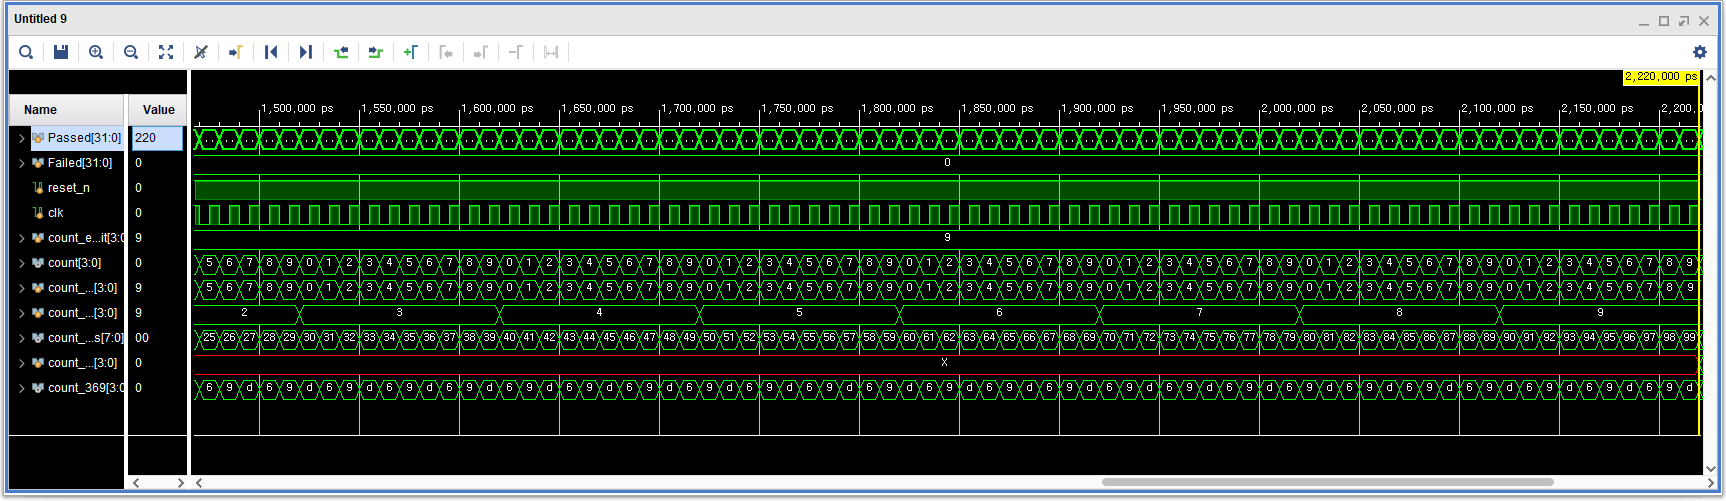
\includegraphics[width=0.9\linewidth]{lab6_2_waveform.png}
\end{figure}
0부터 시작해서 99에 도달한 다음 다시 0으로 돌아가는 정상 작동을 함을 알 수 있다.

\subsection{\texttt{lab6\_3.v} -- 369 계수기}
Vivado에서 생성된 회로는 다음과 같다.
\begin{figure}[H]
  \centering
  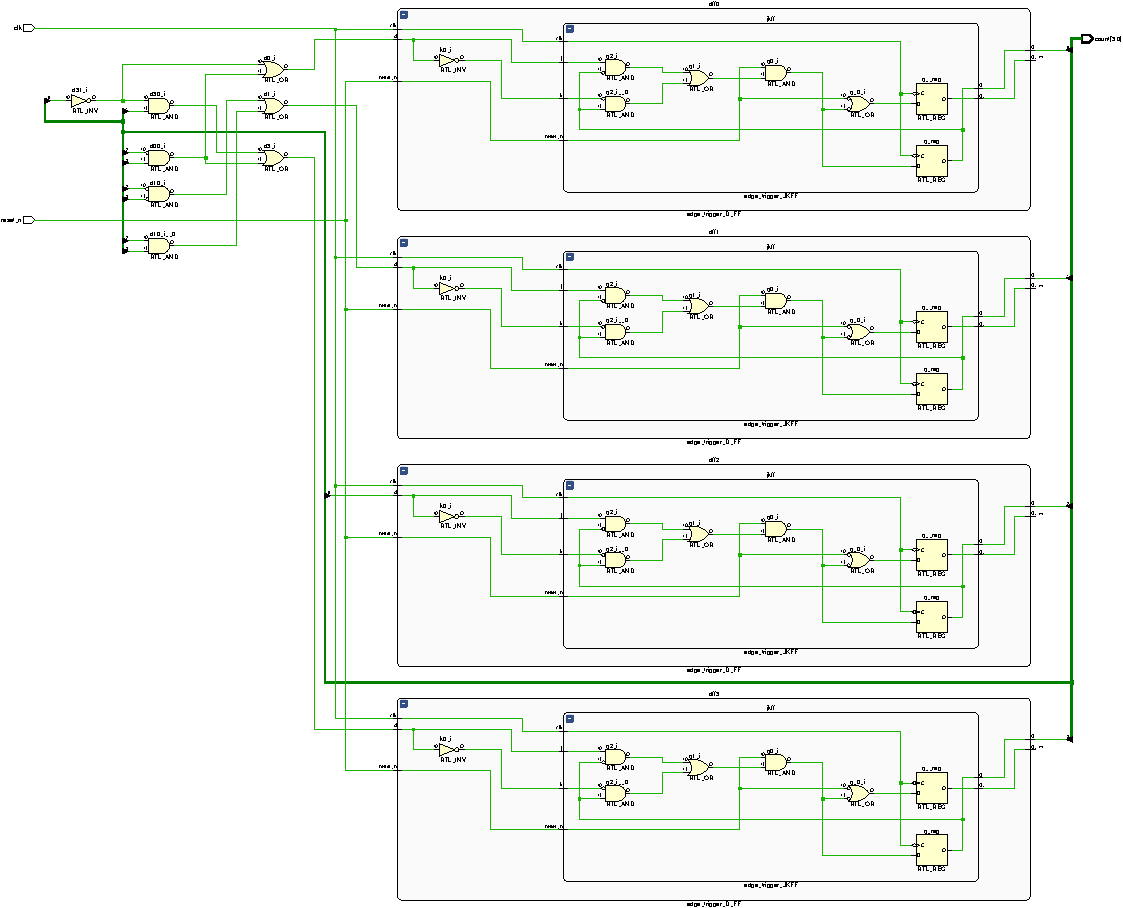
\includegraphics[width=0.9\linewidth]{lab6_3_schematic-crop.pdf}
\end{figure}

테스트벤치 실행 결과 중 \texttt{lab6\_3.v}와 관계있는 부분은 다음과 같다.
\begin{figure}[H]
  \centering
  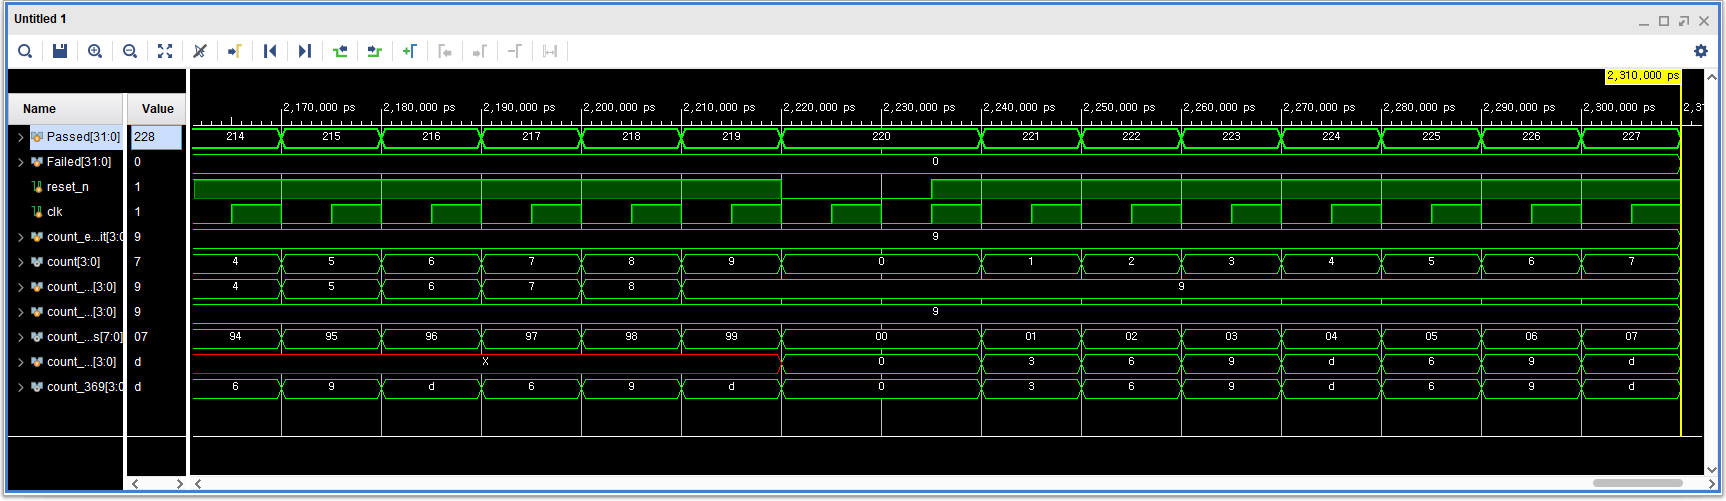
\includegraphics[width=0.9\linewidth]{lab6_3_waveform.png}
\end{figure}
0, 3, 6, 9, 13, 6, 9, \dots 순서로 출력이 나오는 것을 확인할 수 있다.

\section{논의}
수업 시간에 학습한 counter를 직접 구현하고 작동을 확인할 수 있는 시간이었다.
BCD coutner의 경우 수업 시간에는 ripple counter와 비슷한 구조를 보여주었는데, 지금까지 배운 내용으로 synchronous counter를 만든 것이 특히 의미 있었다고 생각한다.

\end{document}
